\chapter{Implementation}

%summarize on what we focused (NVA):
%-high performance
%-reliable
%-ease of use

In the previous chapter we have seen how we approximated the evolution operator. In the following we explain the algorithm that implements the problem.

Our main goal was to develop a high-performance algorithm. The algorithm uses a distribute version of highly optimized CPU and GPU kernels, that runs efficiently on a cluster. Particularly important for this purpose is the memory access pattern optimization. Large amount of data are stored in the main memory. These data need to be sent to the process unit to be processed. Nowadays, process units are by far faster in processing data than the ability of the main memories to fed them. So if the process unit had to fetch data from the main memory, it would be slowed to the velocity of the memory. To avoid this problem we exploit cache-aware computation that uses smaller and faster sub-system memories, dubbed caches. 
Furthermore, a distributed workload across a multiprocessor system requires a communication between the nodes. Indeed, to proceed to the next iteration, a node needs data of the previous iteration calculated by other nodes. The transfer of data in a network of nodes can be even slower than the transfer from main memory to process unit. However, in a certain extent, communication between nodes and calculation in process unit can be done in parallel. For the sake of efficiency, it is worth to overlap the two as much as possible.

For the purpose of developing reliable scientific software, we put emphasis on unit testing. In the development of complex software, it is important to test various part of the code, to be sure of its correctness. A program can be split into several units, each one having a define use and an expected behaviour. Based on this one develop a test to exercise the unit and verify its exactness. We exploit unit testing using the library CppUnit. Moreover, we use double-precision floating point operations, to gain accuracy in the simulations.

Our approach was also to ensure that our implementation fits in with rapid prototyping
systems. The program allows to the use of a command line interface, for the flexibility of the simulation. In addition, the function that performs the evolution is exposed as an application programming interface (API). We also developed wrappers to make the kernels accessible from Python and MATLAB.
%control version system

%kernel citation
Before entering in the details of the algorithm, we explain some concepts important for high performance code.

%%%%%%%%%%%%%%%%%%%%%%%%%%%%%%%%%%%%%%%%%%%%%%%%%%%%%%%%%%%%%%%%%%%%%%%%%%%%%%%%%%%%%%
\section{Cache optimization}
Nowadays there exist a large gap between CPU speed and main memory performance. To alleviate this gap, computer architectures implement hierarchical memory structures. This approach allows to work around both the low main memory bandwidth and the latency of main memory accesses.
The memory bandwidth is a measure of the rate at which data can be read from or stored into the memory by a processor, and it is a crucial parameter that affect an algorithm performance. Along with this factor also the memory latency play an important role in computer performance. The memory latency is the delay time between the moment a memory controller tells the memory module to access a particular memory location, and the moment these data are available on the module's output pins. These parameters characterized the velocity at which the memory can feed the processor. When the CPUs need to process a certain data it request it to the memory. Since that moment it will have to wait the time the date come up to the memory's output pins and the time they take to travel to the CPUs.
 
  The common structure of the hierarchy consist of a series of memories; the smaller they are, the closer they are to the CPUs; the cheaper they are, the further they are from the CPUs. Usually, at the top of the hierarchy there are the registers, memories integrated within the processor chip that can provide data with low latency and high bandwidth. Between the processor core and the main memory there are memories called \emph{cache memories} or \emph{caches}. Finally, there is the main memory, usually constituted of large and slow hard disk drives. During the execution of a program, some blocks of data are used more often than others, so the CPUs will work with this subset of data for most of the time. To get an efficient algorithm, the idea is to store frequently used blocks of data on fast memories: the more frequently the block is used, the higher in the hierarchy is the memory that stores it. 

Typically, the data residing within a smaller memory are also stored within the larger memory, so the levels of the memory hierarchy subset one another. A common memory hierarchy is show in Fig.~\ref{fig:memory-hierarchy}.
\begin{figure}
   \centering
   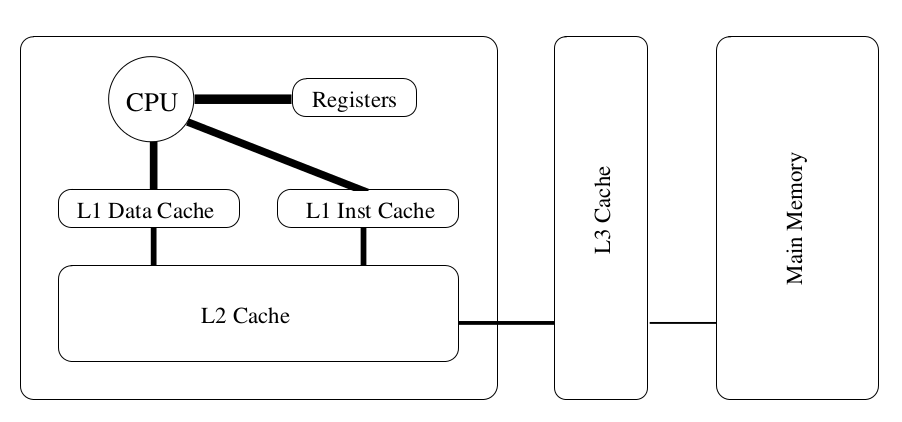
\includegraphics[width=10cm]{Figs/Memory_hierarchy.png}
   \caption{A Common memory hierarchy that present two on-chip L1 caches, on-chip L2 cache, and a third level of off-chip cache. The thickness of the interconnections illustrate the bandwidths between the memory hierarchy levels.} \label{fig:memory-hierarchy}
\end{figure} 

An efficient algorithm must be designed taking care of the memory hierarchical level. Unfortunately, compilers are not intended to introduce sophisticated cache-based transformations. Consequently, the optimization effort is left to the programmer. 

This aspect is particularly important when dealing with numerically intense codes, which occur in science and engineering disciplines, such as computational physics, mechanical engineering and computational fluid dynamic, just to cite some. These type of code are characterized by a large portion of floating-point (FP) operations. Thus, instruction cache misses do not significantly affect the execution performance. Much of the optimization effort concerns data access pattern. Indeed, due to data access latencies and memory bandwidth issues, it is not sufficient to optimize the number of arithmetic operation alone. Efficient codes in scientific computing must necessarily combine computationally optimal algorithms and memory hierarchy optimization.

%%%%%%%%%%%%%%%%%%%%%%%%%%%%%%%%%%%%%%%%%%%%%%%%%%%%%%%%%%%%%%%%%%%%%%%%%%%%%%%%%%%%
\subsection{Organization and Aspects of Cache Architectures}
The common memory hierarchy presents a rather small number of registers on the chip, which has almost no memory latency. On the chip we can also find a small cache -- usually called \textit{level one (L1) cache} -- limited to 64Kbyte, so that low latency and high bandwidth are assured. The latency of \textit{on-chip} caches is commonly one or two CPUs cycles. The L1 cache is often split into two separate parts; one only keeps data, the other instructions. The second level memory (L2) is tipically placed on-chip as well and it is usually limited to 1Mbyte. Due to the bigger size the  latency is around 5 to 10 cycles. Another cache level may be implemented off-chip if the L2 cache is on-chip. The L3 cache size may vary from 1MByte to 16MByte. They provide data with latency of about 10 to 20 cycles.

Data within the cache are stored in \textit{cache lines}. A cache line holds the contents of a contiguous block of main memory. We say that a \textit{cache hit} occur when the data requested by the processor are found in a cache line. If the data requested are not founded in the cache, a \textit{cache miss} occur. In the latter case, the contents of the \textit{memory block} containing the requested words are then fetched from a lower memory layer and copied into a cache line. This operation typically imply another data to be replaced by the new one requested, which is very inefficient. Indeed, the replacement of a cache line takes more time than the CPU to read the same date directly from the main memory. For this reason, caches implement strategy to increase the rate cache hits  over the cache misses. The optimal replacement strategy would be to replace the memory block which will not be accessed for the longest time. However, such strategy is impossible to implement since it requires information about future cache references. 

The most commonly used strategy is \textit{random} and \textit{least recently used (LRU)}. The former randomly chooses a cache line to be replaced. The latter replaces the block which has not been accessed for the longest time interval. Less common strategies are \textit{least frequently used (LFU)} and \textit{first in, first out (FIFO)}. The LFU replaces the memory block in the cache line which has least frequently been used, whereas the FIFO replaces the data which have been residing in cache for the longest time.

These strategy are based on the principle of \textit{locality} references~\cite{Hennessy-Patterson}, which states that recently used data are very likely to be reused in the near future. Locality can be of two different type: \textit{temporal} locality and \textit{spatial} locality. A sequence of references exhibits temporal locality if recently accessed data are likely to be accessed again in the near future. A sequence of references manifest spatial locality if data located close together in address space tend to be referred close together in time.
